\documentclass{beamer}
\usepackage[utf8]{inputenc}
\usetheme{Marburg}

\title{Ecos - Simualtion d'écosystème}
\author{Bastien BONVARLET \and Brandon CHAMPENOIS \and Joris MASSON}
\institute{Université de Caen Normandie}

\begin{document}

\begin{frame}
\titlepage
\end{frame}

\begin{frame}
\tableofcontents
\end{frame}

\section{Présentation générale}
\subsection{En général}

\begin{frame} \frametitle{Éléments généraux}
	\begin{block}{Généralités}
		\begin{itemize}
			\item Une carte sur laquelle évoluent les entités la peuplant(possibilité d'en créer avec Tiled)
			\item Divers type d'entités: 									\begin{itemize}
					\item Humains
					\item Orcs
					\item Loups
					\item Ours
					\item Lapins
				\end{itemize}
			\item Une chaîne alimentaire
		\end{itemize}
	\end{block}
\end{frame}

\subsection{Pourquoi ce choix de projet?}
\begin{frame} \frametitle{Pourquoi ce choix de projet?}
	\begin{block}{Raisons}
		\begin{itemize}
			\item Ça avait l'air sympa
			\item Sujet assez libre
			\item Le sujet le plus inspirant pour nous
		\end{itemize}
	\end{block}
\end{frame}

\section{Répartition des tâches}

\begin{frame} \frametitle{Qui a fait quoi?}
	\subsection{Bastien}
	\begin{block}{Bastien}
		\begin{itemize}
			\item Les différentes cartes
			\item Toute la base du projet
				\begin{itemize}
					\item Les classes
					\item Interface graphique
				\end{itemize}
			\item Tentative de gestion des animations
		\end{itemize}
	\end{block}
	\subsection{Brandon}
	\begin{block}{Brandon}
		\begin{itemize}
			\item Les différents sprites
			\item Le menu de lancement
			\item Le rapport LaTex
		\end{itemize}
	\end{block}
\end{frame}

\begin{frame} \frametitle{Qui a fait quoi?}
	\subsection{Joris}
	\begin{block}{Joris} 
		\begin{itemize}
			\item La programmation de certains aspects du projet:
				\begin{itemize}
					\item L'algorithme A*
					\item Système de combat
					\item Système de reproduction
				\end{itemize}
			\item Création des graphiques
			\item Ce magnifique diaporama en beamer
		\end{itemize}
	\end{block}
\end{frame}

\section{Explication du projet}
\subsection{Général}

\begin{frame} \frametitle{Général}
	\begin{block}{Général}
		\begin{itemize}
			\item Les différentes entités vivent leur vie
				\begin{itemize}
					\item Déplacements aléatoires
					\item Elles s'attaquent entre-elles
					\item Elles peuvent se reproduire
					\item Elles peuvent mourir
						\begin{itemize}
							\item Si leur vie atteint 0
							\item Si elles ont atteint leur âge limite
							\item Si elles sortent de la matrice(belle façon de dire que Joris n'a pas su résoudre un bug)
						\end{itemize}
				\end{itemize}
			\item Le temps passe
				\begin{itemize}
					\item Il passe à un rythme de 60 jours par seconde, un jour par frame
			\item 365 jours dans une année
				\end{itemize}
		\end{itemize}
	\end{block}
\end{frame}

\subsection{Déroulement du programme}

\begin{frame} \frametitle{Déroulement du programme}
	\begin{enumerate}
		\item Initialisation
			\begin{enumerate}
				\item La carte est créée et affichée
				\item Les cases contenant des collisions sont récupérées et stockées pour plus tard
				\item On en déduit les cases n'ayant pas de collisions
				\item On créé un nombre fixe d'entités de manière aléatoire
					\begin{itemize}
						\item Type
						\item Genre
						\item Position
					\end{itemize}
			\end{enumerate}
		\item Les entités font leurs vie, et le monde suit son cours
	\end{enumerate}
\end{frame}

\subsection{Le système de classes}

\begin{frame} \frametitle{Le système de classes}
	\begin{itemize}
		\item Une classe centrale: Game
		\item Une classe mère représentant toutes les entités vivantes: LivingEntity
		\item Une classe mère pour les objets
	\end{itemize}
	\begin{figure}
		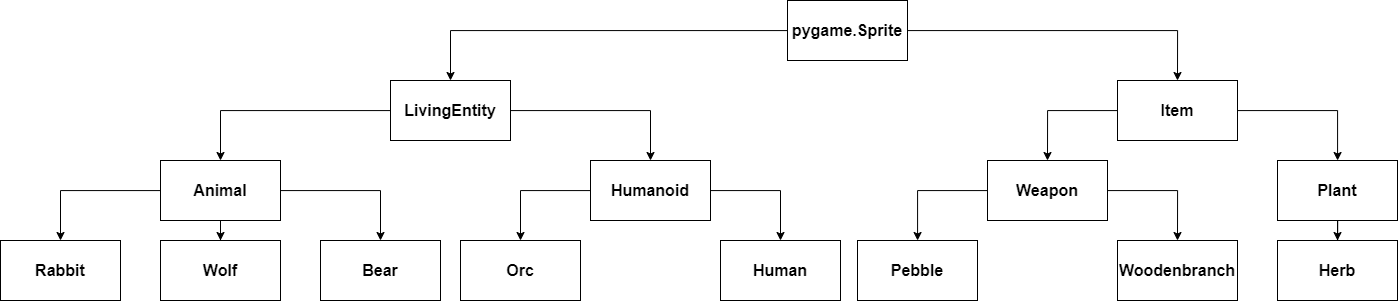
\includegraphics[scale=0.24]{diagramme_class.png}
		\caption{Diagramme de classes}
		\label{Diagramme de classes}
	\end{figure}
\end{frame}

\subsection{Mécaniques}
\subsubsection{Les déplacements}

\begin{frame} \frametitle{Les déplacements}
	\begin{itemize}
		\item Gérés par l'algorithme A*
		\item Destination choisie au hasard
		\item Une fois la destination atteinte, une autre est choisie au hasard
		\item Une seule exécution d'A* par frame par entité
	\end{itemize}
\end{frame}

\subsubsection{Le système de combat}

\begin{frame} \frametitle{Le système de combat}
	\begin{itemize}
		\item Les entités ne peuvent pas se battre avant que le monde ait atteint l'âge de 3 ans
		\item Une attaque survient lorsque deux entités rentrent en contact, et peuvent s'attaquer
		\item Un délai d'attaque est présent(150 frames)
		\item Une attaque a une probabilité de 1/3 d'être initiée par une entité
	\end{itemize}
\end{frame}

\subsubsection{Le système de reproduction}

\begin{frame} \frametitle{Le système de reproduction}
	\begin{itemize}
		\item Le monde doit avoir plus d'un an
		\item Les entités ne peuvent pas se reproduire avant d'avoir atteint un âge minimal spécifique à chaque type d'entité
		\item Ce sont les femelles qui initient la reproduction lorsqu'elle rentre en collision avec une entité du même type, et ayant un genre différent
	\end{itemize}
\end{frame}

\subsubsection{Le système d'arme}

\begin{frame} \frametitle{Le système d'arme}
	\begin{itemize}
		\item Deux types d'armes
		\item Sont à des endroits fixes
		\item Seuls les humanoïdes peuvent s'en servir
		\item Il y a un "temps de recharge"
	\end{itemize}
\end{frame}

\section{Démonstration}

\begin{frame}
	\begin{large}
		\begin{center}
			C'est le moment d'une petite démonstration
		\end{center}
	\end{large}
\end{frame}

\section{Conclusion}
\subsection{Ce qu'on aurait voulu faire}

\begin{frame} \frametitle{Ce qu'on aurait voulu faire}
	\begin{itemize}
		\item Plus d'entités
		\item Des animations
		\item Réparer le lapin
		\item Améliorer le système d'arme
	\end{itemize}
\end{frame}

\subsection{Fin(?)}

\begin{frame} \frametitle{Conclusion}
	\begin{itemize}
		\item Euh
	\end{itemize}
\end{frame}

\end{document}
